\documentclass{article}                     % onecolumn (standard format)
%\documentclass[smallcondensed]{svjour3}     % onecolumn (ditto)
%\documentclass[smallextended]{svjour3}       % onecolumn (second format)
%\documentclass[twocolumn]{svjour3}          % twocolumn
%

\usepackage{geometry}
\usepackage{graphicx}
\usepackage{amsmath}
\usepackage{amsthm}
%\usepackage{mathptmx}
\usepackage{stmaryrd}
\usepackage{enumitem}
\usepackage{times}
\usepackage{graphicx}
\usepackage{latexsym}
\usepackage{bussproofs}
\usepackage{pgf}
\usepackage{adjustbox}
\usepackage{multirow}
\usepackage{array}
\usepackage{tikz}
\usepackage{xcolor}
\usepackage{ushort}
\usepackage{soul}
\usepackage[autostyle]{csquotes}
\usepackage[doi=false,isbn=false,url=false,style=chicago-authordate,natbib=true]{biblatex}

%\usepackage{fonttable}

\addbibresource{KMR_Master.bib}

\newtheorem{theorem}{Theorem}[section]
\newtheorem{corollary}{Corollary}[theorem]
\newtheorem{lemma}[theorem]{Lemma}
\theoremstyle{definition}
\newtheorem{definition}{Definition}[section]


\DeclareMathSymbol{\Gamma}{\mathalpha}{operators}{0}
\DeclareMathSymbol{\Delta}{\mathalpha}{operators}{1}
\DeclareMathSymbol{\Theta}{\mathalpha}{operators}{2}
\DeclareMathSymbol{\Lambda}{\mathalpha}{operators}{3}
\DeclareMathSymbol{\Xi}{\mathalpha}{operators}{4}
\DeclareMathSymbol{\Pi}{\mathalpha}{operators}{5}
\DeclareMathSymbol{\Sigma}{\mathalpha}{operators}{6}
\DeclareMathSymbol{\Upsilon}{\mathalpha}{operators}{7}
\DeclareMathSymbol{\Phi}{\mathalpha}{operators}{8}
\DeclareMathSymbol{\Psi}{\mathalpha}{operators}{9}
\DeclareMathSymbol{\Omega}{\mathalpha}{operators}{10}


\DeclareFontFamily{U} {MnSymbolA}{}

\DeclareFontShape{U}{MnSymbolA}{m}{n}{
  <-6> MnSymbolA5
  <6-7> MnSymbolA6
  <7-8> MnSymbolA7
  <8-9> MnSymbolA8
  <9-10> MnSymbolA9
  <10-12> MnSymbolA10
  <12-> MnSymbolA12}{}
\DeclareFontShape{U}{MnSymbolA}{b}{n}{
  <-6> MnSymbolA-Bold5
  <6-7> MnSymbolA-Bold6
  <7-8> MnSymbolA-Bold7
  <8-9> MnSymbolA-Bold8
  <9-10> MnSymbolA-Bold9
  <10-12> MnSymbolA-Bold10
  <12-> MnSymbolA-Bold12}{}

\DeclareSymbolFont{MnSyA}{U}{MnSymbolA}{m}{n}
\DeclareMathSymbol{\twoheaduparrow}{\mathop}{MnSyA}{25}
\DeclareMathSymbol{\twoheadrightarrow}{\mathop}{MnSyA}{24}

\makeatletter

\usetikzlibrary{shapes}
\usetikzlibrary{fit,shapes.misc}

\newcommand\marktopleft[1]{%
	\tikz[overlay,remember picture] 
	\node (marker-#1-a) at (3cm, 1mm) {};%
}
\newcommand\markbottomright[1]{%
	\tikz[overlay,remember picture] 
	\node (marker-#1-b) at (-3cm,7mm) {};%
	\tikz[overlay,remember picture,thick,inner sep=3pt]
	\node[draw,rounded rectangle,fit=(marker-#1-a.center) (marker-#1-b.center)] {};%
}





\newcommand{\ee}{\twoheadrightarrow}

% % % % % % % % % % % % % % % % Footnote Command % % % % % % % % % % % % %
\usepackage{refcount}% http://ctan.org/pkg/refcount
\newcounter{fncntr}
\newcommand{\fnmark}[1]{\refstepcounter{fncntr}\label{#1}\footnotemark[\getrefnumber{#1}]}
\newcommand{\fntext}[2]{\footnotetext[\getrefnumber{#1}]{#2}}

% % % % % % % % % % % % % % % Internal Commands NMC% % % % % % % % % % % % %
\newcommand{\raisemath}[1]{\mathpalette{\raisem@th{#1}}}
\newcommand{\raisem@th}[3]{\raisebox{#1}{$#2#3$}}

\newcommand{\uuparrow}{% 
	\raisebox{.165ex}{\clipbox{0pt .6pt 0pt 0pt}{$\uparrow$}}
}
\newcommand{\tuuparrow}{% 
	\raisebox{.165ex}{\clipbox{0pt 1pt 0pt 0pt}{$\scriptscriptstyle\uparrow$}}
}
\newcommand{\muparrow}{% 
	\raisebox{.05ex}{\clipbox{0pt .65pt 0pt 0pt}{$\scriptstyle\uparrow$}}
}
\newcommand{\Uuparrow}{% 
	\raisebox{.2ex}{\clipbox{0pt .15pt 0pt 0pt}{$\Uparrow$}}
}
\newcommand{\thuarrow}{% 
	\raisebox{.05ex}{\clipbox{0pt .8pt 0pt 0pt}{$\twoheaduparrow$}}
}

% % % % % COMMANDS FOR NON-MONOTONIC CONSEQUENCES % % % % % % % % %
\newcommand{\nms}{%
	\mathbin{\mathpalette\@nms\expandafter}
}
\newcommand{\@nms}{\mid\joinrel\mkern-.5mu\sim}


\newcommand{\nmc}{%
	\mathbin{\mathpalette\nm@\expandafter}
}
\newcommand{\nm@}{\mid\joinrel\mkern-.5mu\sim\mkern-3mu}

\newcommand{\qmc}[1]{\mathrel{
		\mathchoice
		{\normalsize\hspace{.4mm}\nms^{\mkern-18mu\scriptsize\uuparrow#1}\hspace{-.7mm}}
		{\normalsize\hspace{.4mm}\nms^{\mkern-18mu\scriptsize\uuparrow#1}\hspace{-.7mm}}
		{\footnotesize\hspace{.4mm}\nms^{\mkern-13mu\tiny\uuparrow#1}}
		{\scriptsize\nms^{\mkern-10mu\tiny\tuuparrow#1}}
	}
}

\newcommand{\mqmc}{\mathrel{
		\mathchoice
		{\hspace{.4mm}\nms^{\mkern-18mu\scriptsize\uuparrow}\hspace{.6mm}}
		{\hspace{.4mm}\nms^{\mkern-18mu\scriptsize\uuparrow}\hspace{.6mm}}
		{\footnotesize\hspace{.4mm}\nms^{\mkern-11mu\tiny\uuparrow}\hspace{.6mm}}
		{\scriptsize\nms^{\mkern-10mu\tiny\tuuparrow}}
	}
}

\newcommand{\mrc}[1]{\mathbin{
		\mathchoice
		{\normalsize\hspace{.5mm}\nms^{\mkern-19mu\scriptsize\Uuparrow#1}\hspace{-.5mm}}
		{\normalsize\hspace{.5mm}\nms^{\mkern-19mu\scriptsize\Uuparrow#1}\hspace{-.5mm}}
		{\footnotesize\hspace{.5mm}\nms^{\mkern-13.5mu\fontsize{5.5}{0}\Uuparrow#1}}
		{\scriptsize\nms^{\mkern-10mu\tiny\Uuparrow#1}}
	}
}

\newcommand{\smc}{\mathbin{
		\mathchoice
		{\hspace{.4mm}\nms^{\mkern-17mu\scriptsize\thuarrow}\hspace{.6mm}}
		{\hspace{.4mm}\nms^{\mkern-17mu\scriptsize\thuarrow}\hspace{.6mm}}
		{\footnotesize\hspace{.4mm}\nms^{\mkern-11mu\tiny\thuarrow}\hspace{.6mm}}
		{\scriptsize\nms^{\mkern-10mu\tiny\thuarrow}}
	}
}
\newcommand{\nnmc}{\not\nmc}
\newcommand{\nsmc}{\not\mkern-3mu\smc}
\newcommand{\nmrc}{\not\mkern-3mu\mrc}
\newcommand{\nmqmc}{\not\mkern1mu\mqmc}
\newcommand{\nqmc}{\not\mkern1mu\qmc}

\newcommand{\nme}{%
	\mathbin{\mathpalette\@nme\expandafter}
}
\newcommand{\@nme}{{\mid\joinrel\mkern-.5mu\sim\mkern-2mu}_{e}\mkern3mu}


%\newcommand{\nme}{\nms\mkern-7mu_{e}\mkern2mu}
\newcommand{\qme}{{\qmc\mkern-2mu}_{e}\mkern3mu}
\newcommand{\mqme}{{\mqme\mkern-2mu}_{e}\mkern3mu}
\newcommand{\sme}{{mkern-2mu}_{e}\mkern3mu}

% % % % % % % % % % %Commands for Material Incoherence% % % % % % % % % % % %

\newcommand{\bigperpp}{%
	\mathop{\mathpalette\bigp@rpp\relax}%
	\displaylimits
}
\newcommand{\bigp@rpp}[2]{%
	\vcenter{
		\m@th\hbox{\scalebox{\ifx#1\displaystyle1.15\else1.15\fi}{$#1\perp$}}
	}%
}
\newcommand{\bigperp}{\raisemath{.5pt}{\bigperpp}}

%% % % % % % Degree Command % % % % % % % % % % % % % % % % % % % %
\newcommand{\degree}{\ensuremath{^\circ}}

%%%%%%%%%%%%%Author Comments%%%%%%%%%%%%%%%%%
 \newcommand{\kk}[1]{\textcolor{red}{$^{\textrm{KK}}${#1}}}
 \newcommand{\jm}[1]{\textcolor{blue}{$^{\textrm{JM}}${#1}}}
 \newcommand{\mr}[1]{\textcolor{green}{$^{\textrm{MR}}${#1}}}


\newcolumntype{L}[1]{>{\raggedright\let\newline\\\arraybackslash\hspace{0pt}}m{#1}}
\newcolumntype{C}[1]{>{\centering\let\newline\\\arraybackslash\hspace{0pt}}m{#1}}
\newcolumntype{R}[1]{>{\raggedleft\let\newline\\\arraybackslash\hspace{0pt}}m{#1}}



\makeatother





%\renewcommand{\@cite}[1]{#1}
%\usepackage[natbibapa]{apacite}
\usepackage[hang,flushmargin]{footmisc} 
\usepackage[hidelinks]{hyperref}
%\usepackage{lingmacros}
%\hypersetup{
%    colorlinks=false,
%    pdfborder={0 0 0},
%}


\begin{document}
\sloppy
\title{Pragmatics of Explanation}

\raggedbottom

\maketitle


\noindent\textbf{Quantified Material Consequence (QMC):}\label{QMC}
\begin{equation}
	\Gamma, A \qmc{W} B \Longleftrightarrow_{df}
	\begin{cases}\nonumber
		1.\,\, W\subseteq\mathcal{P}(\mathcal{L}) & $ and $ \\[3pt] 
		2.\,\, \forall\Delta\in W(\Gamma, A,  \Delta \nmc B ) 
	\end{cases}
\end{equation}

\noindent\textbf{Modally Robust Consequence (MRC):}\label{MRC}
\begin{equation}
	\Gamma, A \mrc{W} B \Longleftrightarrow_{df}
	\begin{cases}\nonumber
		1.\,\, \Gamma, A \qmc{W} B& $ and $ \\[3pt] 
		2.\,\, \forall W'(\Gamma, A \qmc{W'} B \Longrightarrow W' \subseteq W)  & $ and $\\[3pt] 
		%3.\,\, \nqmc[]{\Gamma}{B}{W} & $ and $\\[3pt]  
		3.\,\, \forall\Delta(\Gamma, A, \Delta \mqmc \bigperp \Longrightarrow \Delta \not\in W)
		
	\end{cases}
\end{equation}

\noindent\textbf{Sturdy  Consequence (SC): [Sets]}\label{SCset}
\begin{equation}
\Gamma, \, \Sigma \smc B \Longrightarrow
\begin{cases}\nonumber 
1.\,\, \Gamma, \, \Sigma \mrc{W} B & $ where $ B \not\in \Sigma $, and $ \\[3pt] 
2.\,\, \forall \Theta\,(\Gamma, \Theta \mrc{W'} B \Longrightarrow W\not\subset W' ) & $ where $ B\not\in \Theta  \\[3pt] 
\end{cases}
\end{equation}

Let $X, Y, Z$ stand for sets of sets of sentences.

\section{Commitment Space}
%We start with a language, $ \mathcal{L}_e $, conceived as a set consisting of an incoherence constant ($ \bigperp $), atomic sentences, and sentences formed with a connective for non-factive, complete, immediate explanation ($ \ee $). We have already defined material ($ \nmc $), modally robust ($ \mrc{W} $), and sturdy consequence relations ($ \smc $) over this language. We can think of this language as constituting the space of possible commitments that speakers can undertake. Depending on the sentence, these commitments may be doxastic (beliefs) or practical (intentions).

%With the commitment space, speakers collect commitment scores, sets of sentences to which they are committed and to which they take themselves to be entitled.

%\begin{itemize}
%	\item Commitment space is a space where commitments of various flavors can be undertaken: doxastic and practical.
%	\item Sets of commitments can be shared across discourse participants. When that is the case, then the set of commitments represents a conversation context.
%\end{itemize}

%Particular sentences of $ \mathcal{L}_e $ can be evaluated on such a logical space by determining of which maximally coherent sets of sentences they are members.
%[Introduce commitment notion of assertion. ``Brandom has referred to this aspect of the normative force of assertion as an asserter’s ampliative responsibility to extract the consequences of each of her
%commitments in the context of the collateral premises provided by the rest of her
%commitments'' (Brandom 2009, 36-7.).]

%a set, $ Z $, of \textit{maximally coherent sets of sentences }$ $ belonging to  $\mathcal{L}_e $ (MCSs).\fnmark{Zsubset} Equivalently, we can think of the points of this space as MCSs. Formally, we define MCSs as follows:
%\fntext{Zsubset}{Naturally, the commitment space is a proper subset of the power set of the language, i.e. $ Z\subset \mathcal{P}(\mathcal{L}_e) $.}
%\begin{definition}
%	\item A set of sentences, $\Delta$, is maximally materially coherent \textit{iff} $ \Delta $ is materially coherent and there is no proper superset of $ \Delta $ which is materially coherent, i.e. $ \Delta \not\nmc \bigperp $ and $ \Delta \subset \Theta \Longrightarrow \Theta \nmc \bigperp $.
%\end{definition}
%When a speaker asserts a sentence, $ A $ of $ \mathcal{L}_e $ she undertakes a commitment that prohibits her from asserting those MCSS that are incompatible with $ A $. In this sense, asserting $ A $ has the effect of circumscribing the range of future commitments that a speaker is allowed to make. More precisely, a speaker is capable of making subsequent assertions which contradict her previous ones, but she is not \textit{entitled} to do so. (Of course, a speaker may very well retract an assertion and thereby make available those previously impermissible commitments).

%set of sets of sentences compatible with $ \Gamma $, i.e. $ \forall \Delta (\Gamma, \Delta \not\nmc \bigperp ) $. 

We start with a language, $ \mathcal{L}_e $, conceived as a set consisting of an incoherence constant ($ \bigperp $), atomic sentences, and sentences formed with a connective for non-factive, complete, immediate explanation ($ \ee $). We have already defined material ($ \nmc $), modally robust ($ \mrc{W} $), and sturdy consequence relations ($ \smc $) over this language. \jm{Does this need to be extended to include $ \neg $ and $ \wedge $?}

Now, consider the set of all the possible sets of commitments a speaker of a particular language can undertake. Depending on the sentence, these commitments may be assertional or practical (i.e. commitments to perform some action). We can think of this space of possible commitments as the power set of $ \mathcal{L}_e $, i.e. $\mathcal{P}(\mathcal{L}_e) $. If we help ourselves to the metaphor of linguistic practice as a kind of game, then this space of possible commitments is the \textit{game board}. The set of commitments that a speaker has actually undertaken at any point in the game is her \textit{commitment score} at that time. Speaker's commitment scores are represented by the set of sentences to which she has undertaken commitment, e.g. $ \Gamma $.

When a speaker asserts a sentence she makes a certain sort of move in the game. If she asserts $ A $, then she undertakes a commitment that, \textit{inter alia}, prohibits her from asserting those sentences that are incompatible with $ A $. In this sense, asserting $ A $ has the effect of circumscribing the range of future commitments that a speaker is permitted to undertake. Only those sentences with which $A$ is compatible are considered `live options' for future commitment. (Of course, a speaker may very well retract an assertion and thereby make available those previously impermissible commitments). In this sense, we can think of an assertional commitment to $A$ as carving out a portion of the game board consisting of those sets of sentences compatible with $A$. Since it is with this part of the game board that a speaker's entitled commitments are to be found, we call it a speaker's \textit{entitlement space}. Since every assertion a speaker makes alters her entitlement space, and since her total set of commitments is her commitment score, we can say that a speaker's commitment score determines her entitlement space.

We can represent the concepts \textit{game board}, \textit{commitment score}, and \textit{entitlement space} graphically in the following manner.  In the picture below, the rectangle represents the game board and the oval represents the entitlement space for a speaker whose commitment score consists of a single assertional commitment to \textit{A}.  

\begin{center}
	

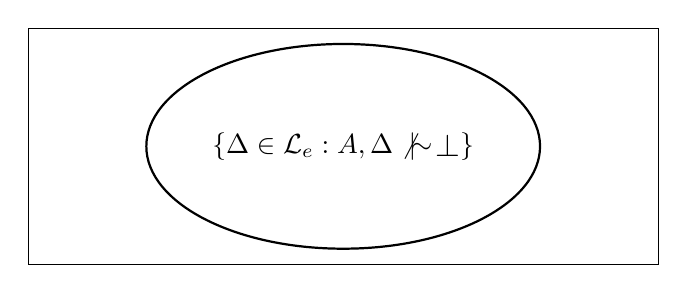
\begin{tikzpicture}

%
\draw[] (0,0)rectangle (8,3);
\draw[thick] (4,1.5) ellipse (2.5 and 1.3);
\draw  (4,1.5) node[]{$ \{\Delta\in\mathcal{L}_e  : A, \Delta \not\nmc \bigperp\} $};
%\tikzstyle{oval} = {ellipse,draw,text width=3cm,align=center}
%\node[xshift=4cm,yshift=2cm,draw,ellipse,text width=3cm,align=center]{{\Large $ \forall \Delta (\Gamma, \Delta \not\nmc \bigperp ) $}};

\end{tikzpicture}

\end{center}


\jm{ \textit{The intersection of the entitlement spaces of all conversational participants constitutes the deontic common ground.} We refer to the set of commitments undertaken by a speaker as her \textit{commitment score} and to the set of commitments shared by the participants of a conversation as the \textit{conversational context} or simply the \textit{context}. (We seem to be assuming perfect transparency of participants commitment scores as well as mutual knowledge. This assumption deserves some discussion)}.



While assertions serve to exclude portions of the commitment space, when a speaker asks a question or \textit{queries} she \textit{partitions} the space of possible commitments. A partition of a set $ Z $ is a set of non-empty subsets of $ Z $ such that the union of those subsets equals $ Z $ and no two of these subsets overlap.

\begin{definition}
\item $ X $ is partition of $ Z $ \textit{iff} $ \forall\Delta \in X: \Delta \neq \emptyset$,$ \bigcup\limits_{\Delta \in X}=  Z$ and $ \forall \Delta \forall \Theta \in X: \Delta \cap \Theta \neq \emptyset \,\Rightarrow\, \Delta = \Theta $.
\end{definition}

To query is to divide up the game board into mutually exclusive sets of sets of sentences and to call upon one's interlocutor's to entitle one to exclude all but one of these sets. In other words, the goal of a query is to determine where one's entitlements lies, which portion of the game board contains those sentences to which a speaker might be entitled. 

To illustrate the effect that queries have on commitment space, we introduce an operator, ?, that takes sets of sentences as arguments. The partition of commitment space induced by the formula $ ?\{A\} $ is represented in the following picture:

\begin{center}
	

\begin{tikzpicture}

%
%\node[draw,rectangle,text width=3cm,align=center]{};
\draw[] (0,0)rectangle (4,3);
\draw  (2,1.5) node[]{$ \{\Delta : A, \Delta \not\nmc \bigperp\} $};
\draw[] (4,0)rectangle (8,3);
\draw  (6,1.5) node[]{$ \{\Delta : A, \Delta \nmc \bigperp\} $};
%\draw[thick] (5,2.5) ellipse (3 and 2);
%\tikzstyle{oval} = {ellipse,draw,text width=3cm,align=center}
%\node[xshift=4cm,yshift=2cm,draw,ellipse,text width=3cm,align=center]{{\Large $ \forall \Delta (\Gamma, \Delta \not\nmc \bigperp ) $}};

\end{tikzpicture}

\end{center}

Likewise, the following picture represents the partition of commitment space induced by the question $ ?\{A,B\} $:



\begin{center}
\renewcommand{\arraystretch}{4}
\begin{tabular}{|c|c|}
\hline 
 $ \{\Delta : A, \Delta \not\nmc \bigperp\} \,\,\bigcap\,\, \{\Delta : B, \Delta \not\nmc \bigperp\} $ & $ \{\Delta : A, \Delta \nmc \bigperp\}  \,\,\bigcap\,\, \{\Delta : B, \Delta \not\nmc \bigperp\} $  \\ 
\hline 
$ \{\Delta : A, \Delta \not\nmc \bigperp\} \,\,\bigcap\,\, \{\Delta : B, \Delta \nmc \bigperp\} $ & $ \{\Delta : A, \Delta \nmc \bigperp\}  \,\,\bigcap\,\, \{\Delta: B, \Delta \nmc \bigperp\} $  \\ 
\hline 
\end{tabular} 
\end{center}





%\begin{center}
%\renewcommand{\arraystretch}{4}
%\begin{tabular}{|c|c|}
%\hline 
% $ \forall \Delta (A, \Delta \not\nmc \bigperp ) \,\,\bigcap\,\, \forall \Delta (B, \Delta \not\nmc \bigperp ) $ & $ \forall \Delta (A, \Delta \nmc \bigperp )  \,\,\bigcap\,\, \forall \Delta (B, \Delta \not\nmc \bigperp ) $  \\ 
%\hline 
%$ \forall \Delta (A, \Delta \not\nmc \bigperp )  \,\,\bigcap\,\, \forall \Delta (B, \Delta \nmc \bigperp ) $ & $ \forall \Delta (A, \Delta \nmc \bigperp )  \,\,\bigcap\,\, \forall \Delta (B, \Delta \nmc \bigperp ) $  \\ 
%\hline 
%\end{tabular} 
%\end{center}

%%
%\begin{tabular}{|c|c|}
%\hline 
%$ \forall \Delta (A, \Delta \not\nmc \bigperp ) $ and $ \forall \Delta (B, \Delta \not\nmc \bigperp ) $ & $ \forall \Delta (A, \Delta \nmc \bigperp ) $ and $ \forall \Delta (B, \Delta \not\nmc \bigperp ) $
%\hline 
%$ \forall \Delta (A, \Delta \not\nmc \bigperp ) $ and $ \forall \Delta (B, \Delta \nmc \bigperp ) $ & $ \forall \Delta (A, \Delta \nmc \bigperp ) $ and $ \forall \Delta (B, \Delta \nmc \bigperp ) $ \\ 
%\hline 
%\end{tabular} 
%%\renewcommand{\arraystretch}{4}
%\begin{tabular}{|c|c|}
%\hline 
%$ \forall \Delta (A, \Delta \not\nmc \bigperp ) $ & $ \forall \Delta (A, \Delta \nmc \bigperp ) $ 
% 
%$ \forall \Delta (B, \Delta \not\nmc \bigperp ) $ & $ \forall \Delta (B, \Delta \not\nmc \bigperp ) $
%\hline 
%$ \forall \Delta (A, \Delta \not\nmc \bigperp ) $ & $ \forall \Delta (A, \Delta \nmc \bigperp ) $ \\ 
%$ \forall \Delta (B, \Delta \nmc \bigperp ) $ & $ \forall \Delta (B, \Delta \nmc \bigperp ) $
%\hline 
%\end{tabular} 


%The force of a query is to call upon one's interlocutors to determine which areas (cells of the partition) of commitment space 







\vspace{3cm}

\section{Desiderata for a Pragmatics of Explanation:}
\begin{itemize}
\item Account for the difference between logically possible answers to a why-question and the contextually possible answers  to a why-question.
\item Treat the propriety of contextually possible answers as a function of the cognitive and conative states/attitudes (or their deontic scorekeeping analogs) of conversational participants.
\item If the alternatives that comprise the semantic content of why-questions are complete explanations, then the pragmatics needs to provide a notion of a \textit{partial answer to a why-Question} as well as the rules that govern which partial answers are the `right ones' given the context (see next point).
\item Define the relationship between complete/partial explanations and complete/partial answers to why-questions.
\item Identify the contextual parameters that determine what makes an explanation (i.e.possible [partial] answer to a why-question) the `best'.
\item Make our picture of explanatory practices more descriptively adequate.
\item Less urgent:
\begin{itemize}
\item Account for the impermissibility of disjunctive explanations.
\item Account for distinction between A and Gamma??
\end{itemize}
\end{itemize}


\section{Initial Thoughts:}
\begin{itemize}
\item \textsc{Hypothesis:} Sturdy inferences ($\Gamma, \Sigma \smc B $) are made explicit by claims of non-factive, complete, immediate explanation ($\Gamma, \Sigma \ee B $).
\begin{itemize}
\item \textit{Non-factive:} A sturdy inference entails neither the explanans nor the explanadum.
\item \textit{Complete:} Nothing need be added to $\Sigma$ in the context of $\Gamma$ in order to explain $B$.
\item \textit{Immediate:} It is not the case that $\Sigma$ explains $B$ in $\Gamma$ by explaining some $C$ which then explains $B$. 
\end{itemize}

\item The set of alternatives which constitutes or in part constitutes the semantic content of why-questions, e.g. \textit{Why B?} are NOT the premises of sturdy inferences (i.e. $\Sigma$), but are the inferences, or the explicit inferential commitments themselves (i.e. $\Gamma, \Sigma \ee B $) with the same conclusion.
\begin{itemize}
\item[***] \textbf{Are the alternatives (1) sturdy inferences (i.e. $\Gamma, \Sigma \smc B \,\,$; $\,\,\Gamma \Theta \smc B $ ; etc.) or (2) merely modally robust inferences (i.e. $\Gamma, \Sigma \mrc{W} B \,\,$; $\,\,\Gamma, \Theta \mrc{W'} B $ ; etc.)?}
\begin{itemize}
\item Option (1) would be in keeping with the standard semantics for questions, but (2) would align with our SC2...
\item Let's go with option (1) and see how far we can run with it.\\
\end{itemize}
\end{itemize}
\end{itemize}

\section{Intro to Partition Semantics and Pragmatics of Answers}

In their dissertation, Groenendijk and Stokhof, provide a partition semantics for questions and a pragmatics for answers. The basic idea is that the semantic content of questions is a partition on logical space that divides the latter into mutually exclusive, exhaustive possibilities. For instance, the question ``Who's in Chicago'' ($ ?xCx $) asked in universe of discourse consisting of only two individuals, \textit{a} and \textit{b}, would divide logical space as follows:

\renewcommand{\arraystretch}{4}
\begin{tabular}{ r|C{4cm}|C{4cm}| }
	\multicolumn{1}{r}{}
	&  \multicolumn{1}{c}{$Ca$}
	& \multicolumn{1}{c}{$\neg Ca$} \\
	\cline{2-3}
	$Cb$ & $Ca \wedge Cb$ & $\neg Ca \wedge Cb$ \\
	\cline{2-3}
	$\neg Cb$ & $Ca \wedge \neg Cb$ & $\neg Ca \wedge \neg Cb$ \\
	\cline{2-3}
\end{tabular}\\

A complete answer to a question is a piece of information that identifies one cell as actual, while a partial answer is any piece of information that permits us to eliminate at least one cell. 

G \& S's pragmatics aims to represent the role that context plays in circumscribing the set of possible answers. If the context is a set of propositions, then the pragmatically relevant possible answers as those that partition the portion of logical space carved out by the context. Consider the following picture, the same as the one for $ ?xCx $, but now with an additional oval which represents the current state of information, i.e. the context:

\renewcommand{\arraystretch}{4}
\begin{tabular}{ r|L{4cm}|R{4cm}| }
	\multicolumn{1}{r}{}
	&  \multicolumn{1}{c}{$Ca$}
	& \multicolumn{1}{c}{$\neg Ca$} \\
	\cline{2-3}
	$Cb$ &	\marktopleft{c1}\raisebox{.7cm}{$Ca \wedge Cb$}
	& \raisebox{.7cm}{$\neg Ca \wedge Cb$} \\
	\cline{2-3}
	$\neg Cb$ & $Ca \wedge \neg Cb$ & $\neg Ca \wedge \neg Cb$\markbottomright{c1} \\
	\cline{2-3}
\end{tabular}\\

\vspace{3mm}

The oval represents the idea that participants assume that actual world lies inside of it, and that all possibilities outside the oval have been dismissed as being non-actual. (Of course, it may be that they have been dismissed mistakenly.) The above picture indicates that, while the semantic question cuts up logical space into four big blocks, it is the division of the oval into four parts that is pragmatically relevant. 

Of course, context can also exclude certain logically possible answers, i.e. exclude cells of the partition of logical space. The next picture represents a context that excludes certain alternatives.

\renewcommand{\arraystretch}{4}
\begin{tabular}{ r|L{4cm}|R{4cm}| }
	\multicolumn{1}{r}{}
	&  \multicolumn{1}{c}{$Ca$}
	& \multicolumn{1}{c}{$\neg Ca$} \\
	\cline{2-3}
	$Cb$ &	\marktopleft{c1}\raisebox{.7cm}{$Ca \wedge Cb$}
	& \raisebox{.7cm}{$\neg Ca \wedge Cb$}\markbottomright{c1}  \\
	\cline{2-3}
	$\neg Cb$ & $Ca \wedge \neg Cb$ & $\neg Ca \wedge \neg Cb$ \\
	\cline{2-3}
\end{tabular}\\

\vspace{2mm}
In this scenario, only two of the logically possible answers are permissible in the context.

\section{Applying Partition Semantics to Why-questions:}

The first step in articulating a partition semantics for why-questions is to determine how why-questions partition logical space. Our guiding insight is that why-questions divide logical space into possible complete explanations.  However, while we have been representing complete explanations as sturdy inferences relativized to contexts (i.e. $\Gamma$), we should omit these contexts in our formalization of the partition induced by why-questions since the semantics already has a mechanism for representing contexts. Thus, the set of alternative associated with the question \textit{Why B?} is $ \{ \Sigma \ee B \,\,,\,\, \Theta \ee B \} $ rather than $\{ \Gamma, \Sigma \ee B \,\,$; $\,\,\Gamma, \Theta \ee B \} $. Following the partition semantics approach, the semantic content of this question is the partition induced by this set, i.e. the set of mutually-exclusive, exhaustive possibilities: $$ \{ \Sigma \ee B  \,\,\&\,\, \Theta \ee B,\,\, \Sigma \ee B \,\,\&\,\,\neg(\Theta \ee B),\,\, \neg(\Sigma \ee B) \,\,\&\,\,\Theta \ee B,\,\, \neg(\Sigma \ee B)\,\,\&\,\,\neg(\Theta \ee B)       \} $$  

The partition looks like this:\\

\renewcommand{\arraystretch}{4}
\begin{tabular}{ r|C{4cm}|C{4cm}| }
	\multicolumn{1}{r}{}
	&  \multicolumn{1}{c}{$\Sigma \ee B$}
	& \multicolumn{1}{c}{$\neg(\Sigma \ee B)$} \\
	\cline{2-3}
	$\Theta \ee B$ & $\Sigma \ee B \,\,$ \& $\,\,\Theta \ee B$ & $\neg(\Sigma \ee B) \,\,\&\,\, \Theta \ee B$ \\
	\cline{2-3}
	$\neg(\Theta \ee B)$ & $\Sigma \ee B \,\,$ \& $\,\,\neg(\Theta \ee B)$ & $\neg(\Sigma \ee B)\,\,\&\,\,\neg(\Theta \ee B)$ \\
	\cline{2-3}
\end{tabular}\\




%\renewcommand{\arraystretch}{3}
%\begin{tabular}{|c|c|}
%\hline $ \Sigma \ee B \,\,$ \& $\,\,\Theta \ee B $
% & $ \Sigma \ee B \,\,$ \& $\,\,\neg(\Theta \ee B) $ \\ 
%\hline $ \neg(\Sigma \ee B) \,\,\&\,\, \Theta \ee B $
% & $ \neg(\Sigma \ee B)\,\,\&\,\,\neg(\Theta \ee B) $ \\ 
%\hline 
%\end{tabular} \\\\

\vspace{3mm}

Now here is the same question, \textit{Why B?} asked in context $\Gamma$. Here, the oval represents the set of commitments $\Gamma$.

\renewcommand{\arraystretch}{4}
\begin{tabular}{ r|C{4cm}|C{4cm}| }
	\multicolumn{1}{r}{}
	&  \multicolumn{1}{c}{$\Sigma \ee B$}
	& \multicolumn{1}{c}{$\neg(\Sigma \ee B)$} \\
	\cline{2-3}
	$\Theta \ee B$ & \marktopleft{c1}\raisebox{.7cm}{$\Sigma \ee B \,\,$ \& $\,\,\Theta \ee B$} & \raisebox{.7cm}{$\neg(\Sigma \ee B) \,\,\&\,\, \Theta \ee B$} \\
	\cline{2-3}
	$\neg(\Theta \ee B)$ & $\Sigma \ee B \,\,$ \& $\,\,\neg(\Theta \ee B)$ & $\neg(\Sigma \ee B)\,\,\&\,\,\neg(\Theta \ee B)$\markbottomright{c1} \\
	\cline{2-3}
\end{tabular}\\

\vspace{5mm}

Just as in the case of \textit{Who}-question, why-questions can be asked in contexts in which some logically possible answers are not contextually permissible. In the case of why-questions, this means that certain possible complete explanations are excluded from consideration.

\renewcommand{\arraystretch}{4}
\begin{tabular}{ r|C{4cm}|C{4cm}| }
	\multicolumn{1}{r}{}
	&  \multicolumn{1}{c}{$\Sigma \ee B$}
	& \multicolumn{1}{c}{$\neg(\Sigma \ee B)$} \\
	\cline{2-3}
	$\Theta \ee B$ & \raisebox{.7cm}{$\Sigma \ee B \,\,$ \& $\,\,\Theta \ee B$}\marktopleft{c1} & \raisebox{.7cm}{$\neg(\Sigma \ee B) \,\,\&\,\, \Theta \ee B$} \\
	\cline{2-3}
	$\neg(\Theta \ee B)$ & $\Sigma \ee B \,\,$ \& $\,\,\neg(\Theta \ee B)$ & $\neg(\Sigma \ee B)\,\,\&\,\,\neg(\Theta \ee B)$\markbottomright{c1} \\
	\cline{2-3}
\end{tabular}\\

\vspace{5mm}

In this situation, the context, $\Sigma$ is not a permissible answer to the question \textit{Why B?}, and hence is not a competitor for the status of complete explanation of $B$.

\section{Pragmatics of Answers and Explanation}

Recall that in partition semantics for questions, a partial answer is any piece of information that permits us to eliminate at least one cell. So, any of the following would be a partial answer to the question ``Why B?'' asked in $\Gamma$: e.g. $\Sigma \ee B\,,\,\, \neg(\Theta \ee B)\,,\,\, \neg(\Sigma \ee B)\,,\,\, \Theta \ee B  $. 

But in most conversational contexts, we answer why questions by giving only a partial explanation. In fact, complete explanations seem to be very rarely called for. Given, the way we have defined \textit{partial answer to a why-question}, we can say that \textbf{a partial explanation is a part of a partial answer to a why-question.} For example, to the question ``Why B?'' a normal response would be ``Because A'' where $ A \in \Sigma $. In a context that includes all the cells of the partition above, this response will conversationally entail the partial answer $\Sigma \ee B  $.\\

\textbf{Definition:} A partial explanation of B is a part of a partial answer to the question ``Why B?''\\

\begin{itemize}
	\item A big difference between our pragmatics and that of G\&S is that we conceive of context as a set of commitments (and entitlements?) that consists of both the doxastic and the practical variety. (Perhaps also erotetic and apokritic).
	\item We can successfully do so because we are working on the basis of material inferences and there are certainly practical material inferences.
\end{itemize}

******Gamma weeds out alternative explanations by restricting the sets of suppositions that may be added to the material inferences. This follows from MR3*****












%\noindent\textbf{Context-Set}\\
%\noindent $  \Pi \in \mathcal{L}   $\\


%\noindent\textbf{Sturdy  Consequence (SC):}\label{SC}
%\begin{equation}
%	\Gamma, \,A \smc B \Longrightarrow
%	\begin{cases}\nonumber 
%		1.\,\, \Gamma, \, A \mrc{W} B & $ where $ A \neq B $, and $ \\[3pt] 
%		2.\,\, \forall C\,(\Gamma, C \mrc{W'} B \Longrightarrow W\not\subset W' ) & $ where $ B\neq C  \\[3pt] 
%	\end{cases}
%\end{equation}
%
%\noindent\textbf{Sturdy  Consequence (SC): [Sets]}\label{SCset}
%\begin{equation}
%\Gamma, \, \Sigma \smc B \Longrightarrow
%\begin{cases}\nonumber 
%1.\,\, \Gamma, \, \Sigma \mrc{W} B & $ where $ B \not\in \Sigma $, and $ \\[3pt] 
%2.\,\, \forall \Theta\,(\Gamma, \Theta \mrc{W'} B \Longrightarrow W\not\subset W' ) & $ where $ B\not\in \Theta  \\[3pt] 
%\end{cases}
%\end{equation}



\printbibliography


\end{document}
